\documentclass[twocolumn,a4]{article}
\usepackage{amsmath}
\usepackage{multicol}
\usepackage{tikz}
\usepackage[margin=0.5in]{geometry}

\pagestyle{empty} % Remove page numbers

\begin{document}

\subsubsection*{1. Properties of Equality}
\begin{align*}
\text{Reflexive} \quad & a = a \\
\text{Symmetric} \quad & \text{If } a = b, \text{ then } b = a \\
\text{Transitive} \quad & \text{If } a = b \text{ and } b = c, \text{ then } a = c
\end{align*}

\subsubsection*{2. Properties of Addition and Multiplication}
\begin{align*}
\text{Commutative} \quad & a + b = b + a \text{ , } a * b = b * a \\
\text{Associative} \quad & (a + b) + c = a + (b + c) \\
\quad & (a * b) * c = a * (b * c) \\
\text{Neutral element} \quad & a + 0 = a \text{ , } a * 1 = a \\
\text{Inverse} \quad & \forall a , \exists (-a) : a + (-a) = 0 \\
\quad & \forall a \neq 0 , \exists a^{-1} : a * a^{-1} = 1 \\
\text{Zero} \quad & a \times 0 = 0 \\
\text{Distribution} \quad & a \times (b + c) = a \times b + a \times c
\end{align*}

\subsubsection*{3. Exponent Rules}
\begin{align*}
\text{Product of Powers} \quad & a^m \times a^n = a^{m+n} \\
\text{Power of a Power} \quad & (a^m)^n = a^{m \times n} \\
\text{Power of a Product} \quad & (a \times b)^n = a^n \times b^n \\
\text{Quotient of Powers} \quad & \frac{a^m}{a^n} = a^{m-n} \quad \text{(for } a \neq 0\text{)} \\
\text{Zero Exponent} \quad & a^0 = 1 \quad \text{(for } a \neq 0\text{)} \\
\text{Negative Exponent} \quad & a^{-n} = \frac{1}{a^n} \quad \text{(for } a \neq 0\text{)} \\
\text{Fractional Exponent} \quad & a^{\frac{1}{n}} = \sqrt[n]{a}
\end{align*}

\subsubsection*{4. Special Products}
\begin{align*}
(a + b)^2 &= a^2 + 2ab + b^2 \\ 
(a - b)^2 &= a^2 - 2ab + b^2 \\
a^2 - b^2 &= (a + b)(a - b) \\
\end{align*}

\subsubsection*{5. Quadratic Formula}
\begin{align*}
\text{Given} \quad & a * x^2 + b * x + c = 0 \\
\text{Roots} \quad & x = \frac{-b \pm \sqrt{b^2 - 4ac}}{2a}
\end{align*}

\subsubsection*{6. Series}
\begin{align*}
\text{Arithmetic Term formula} \quad & t_n = a * n + b\\
\text{Sum of first n} \quad & S_n = \frac{n}{2} ( t_1 + t_n )  = \frac{n}{2} \left(a(n + 1) + 2b\right) \\
\text{Geometric Term formula} \quad & a_n = a \cdot r^{n-1} \\
\text{Sum of first n} \quad & S_n = \frac{a(1 - r^n)}{1 - r} \quad \text{for } r \neq 1 \\
\end{align*}

\subsubsection*{7. Trigonometry}
SOHCAHTOA
\begin{tikzpicture}[scale=0.5, overlay, shift={(10cm,0)}]
  % Draw the unit circle
  \draw (0,0) coordinate (O) circle [radius=3cm];

  % Draw the axes
  \draw[->] (-3.2,0) -- (3.2,0) node[right] {$X$};
  \draw[->] (0,-3.2) -- (0,3.2) node[above] {$Y$};
  
  % Draw the sine line
  \draw[red, very thick] (30:3cm) coordinate (A)
  -- (0,0-|A) coordinate(Ax) 
  node[midway,left]{$\sin\alpha$};
  
  % Draw the tangent line
  \draw [very thick, orange] (3,0) -- (intersection cs:
  first line={(O)--(A)},second line={(3,0)--(3,3)}) coordinate(A')
  node[midway,right]{$\tan\alpha$};
  
  % Draw the angle arc and label it
  \draw[thick] (Ax) arc[start angle=0, end angle=30, radius=0.5cm];
  \node at (1.5,0.5) {$\alpha$};
  
  % Draw the line OA'
  \draw (O) -- (A');
  
  % Draw the cosine line
  \draw[very thick, blue] (O) -- (Ax) node[midway,below]{$\cos\alpha$};
\end{tikzpicture}
\\
\\
\begin{align*}
\sin^2(x) + \cos^2(x) &= 1 \\
\sin(a \pm b) &= \sin(a)\cos(b) \pm \cos(a)\sin(b) \\
\cos(a \pm b) &= \cos(a)\cos(b) \mp \sin(a)\sin(b) \\
\tan(a \pm b) &= \frac{\tan(a) \pm \tan(b)}{1 \mp \tan(a)\tan(b)} \\
\sin(2x) &= 2\sin(x)\cos(x) \\
\cos(2x) &= \cos^2(x) - \sin^2(x) \\
\quad &= 2\cos^2(x) - 1 = 1 - 2\sin^2(x) \\
\tan(2x) &= \frac{2\tan(x)}{1 - \tan^2(x)}
\end{align*}

\subsubsection*{8. Logarithm Rules}
\begin{align*}
\text{Product} \quad & \log_b(xy) = \log_b(x) + \log_b(y) \\
\text{Quotient} \quad & \log_b\left(\frac{x}{y}\right) = \log_b(x) - \log_b(y) \\
\text{Power} \quad & \log_b(x^y) = y \log_b(x) \\
\text{Change of Base} \quad & \log_b(x) = \frac{\log_k(x)}{\log_k(b)}
\end{align*}

\subsubsection*{9. Differentiation}
\begin{align*}
\frac{d}{dx}(u(x)+v(x)) &= \frac{d}{dx}u(x) + \frac{d}{dx}v(x) \\
\frac{d}{dx}(c \cdot u(x)) &= c \cdot \frac{d}{dx}u(x) \\
\frac{d}{dx}(u(x) \cdot v(x)) &= \left(\frac{d}{dx}u(x)\right)v(x) + u(x)\left(\frac{d}{dx}v(x)\right) \\
\frac{d}{dx}\left(\frac{u(x)}{v(x)}\right) &= \frac{\left(\frac{d}{dx}u(x)\right)v(x) - u(x)\left(\frac{d}{dx}v(x)\right)}{(v(x))^2} \\
\frac{d}{dx}(x^n) &= n \cdot x^{n-1} \\
\frac{d}{dx}(u(v(x))) &= \left(\frac{d}{dx}u(x)\right)(v(x)) \cdot \left(\frac{d}{dx}v(x)\right)
\end{align*}

\subsubsection*{10. Derivatives of Basic Functions}

\begin{multicols}{2}
\begin{align*}
\frac{d}{dx}(\sin x) &= \cos x \\
\frac{d}{dx}(\cos x) &= -\sin x \\
\frac{d}{dx}(\tan x) &= \sec^2 x \\
\frac{d}{dx}(\cot x) &= -\csc^2 x \\
\end{align*}
\columnbreak
\begin{align*}
\frac{d}{dx}(\sec x) &= \sec x \tan x \\
\frac{d}{dx}(\csc x) &= -\csc x \cot x \\
\frac{d}{dx}(e^x) &= e^x \\
\frac{d}{dx}(\ln x) &= \frac{1}{x}
\end{align*}
\end{multicols}

\subsubsection*{11. Area Circumference etc.}

Triangle \\
\begin{minipage}{0.5\linewidth}
    \begin{itemize}
        \item Base: $b$, Height: $h$
        \item Perimeter: $P = a + b + c$
        \item Area: $A = \frac{1}{2} b h$
    \end{itemize}
\end{minipage}
\begin{minipage}{0.4\linewidth}
    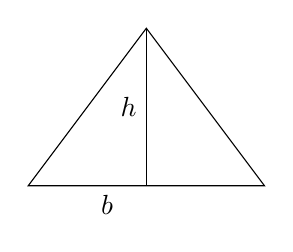
\begin{tikzpicture}
        \draw (0,0) -- (3,0) -- (1.5,2) -- cycle;
        \draw (1.5, 0) -- (1.5, 2);
        \node[below] at (1,0) {$b$};
        \node[left] at (1.5,1) {$h$};
    \end{tikzpicture}
\end{minipage}

Square \\
\begin{minipage}{0.4\linewidth}
	\begin{itemize}
	    \item Side length: $s$
	    \item Perimeter: $P = 4s$
	    \item Area: $A = s^2$
	\end{itemize}
\end{minipage}
\begin{minipage}{0.4\linewidth}
    \begin{tikzpicture}
        \draw (0,0) rectangle (2,2);
        \node[above] at (1,2) {$s$};
        \node[right] at (2,1) {$s$};
    \end{tikzpicture}
\end{minipage}

Rectangle \\
\begin{minipage}{0.4\linewidth}
	\begin{itemize}
	    \item Width: $w$, Height: $h$
	    \item Perimeter: $P = 2(w + h)$
	    \item Area: $A = wh$
	\end{itemize}
\end{minipage}
\begin{minipage}{0.4\linewidth}
    \begin{tikzpicture}
        \draw (0,0) rectangle (3,2);
        \node[above] at (1.5,2) {$w$};
        \node[right] at (3,1) {$h$};
    \end{tikzpicture}
\end{minipage}


Parallelogram \\
\begin{minipage}{0.4\linewidth}
    \begin{itemize}
        \item Base: $b$, Height: $h$
        \item Perimeter: $P = 2(a + b)$
        \item Area: $A = b h$
    \end{itemize}
\end{minipage}
\begin{minipage}{0.4\linewidth}
    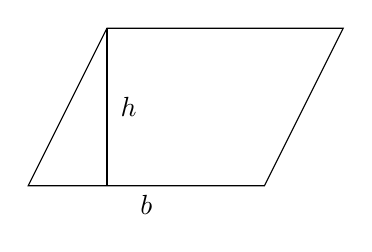
\begin{tikzpicture}
        \draw (0,0) -- (3,0) -- (4,2) -- (1,2) -- cycle;
        \draw (1,0) -- (1,2);
        \node[below] at (1.5,0) {$b$};
        \node[left] at (1.5,1) {$h$};
    \end{tikzpicture}
\end{minipage}

Trapezoid \\
\begin{minipage}{0.4\linewidth}
    \begin{itemize}
        \item Bases: $b_1, b_2$, Height: $h$
        \item Perimeter: $P = a + b_1 + b_2 + c$
        \item Area: $A = \frac{1}{2} (b_1 + b_2) h$
    \end{itemize}
\end{minipage}
\begin{minipage}{0.4\linewidth}
    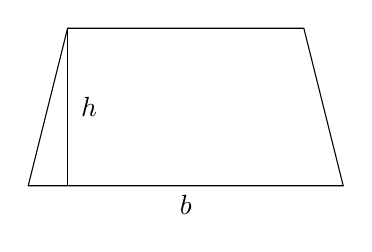
\begin{tikzpicture}
        \draw (0,0) -- (4,0) -- (3.5,2) -- (0.5,2) -- cycle;
        \draw (0.5,0) -- (0.5,2);
        \node[below] at (2,0) {$b$};
        \node[left] at (1,1) {$h$};
    \end{tikzpicture}
\end{minipage}


Circle \\
\begin{minipage}{0.4\linewidth}
	\begin{itemize}
	    \item Radius: $r$
	    \item Circumference: $C = 2\pi r$
	    \item Area: $A = \pi r^2$
	\end{itemize}
\end{minipage}
\begin{minipage}{0.4\linewidth}
    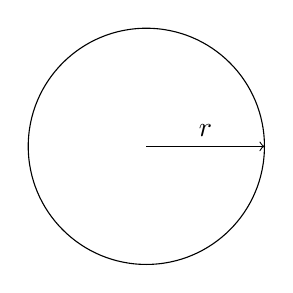
\begin{tikzpicture}
        \draw (0,0) circle (1.5);
        \draw[->] (0,0) -- (1.5,0);
        \node[above] at (0.75,0) {$r$};
    \end{tikzpicture}
\end{minipage}


\end{document}
